\documentclass[12pt, dvipsnames, svgnames, x11names,]{article}

\usepackage{xcolor}
% URLs and hyperlinks ---------------------------------------
\usepackage{hyperref}
\hypersetup{
    colorlinks=true,
    linkcolor=NavyBlue,
    filecolor=magenta,      
    urlcolor=blue,
}
\usepackage{xurl}
%---------------------------------------------------
\usepackage[inline]{enumitem}
\usepackage{graphicx}
\usepackage{multirow}
\usepackage{float}
\renewcommand{\arraystretch}{1.40}

% adjust a verrrrry big table -------------------------------
\usepackage{adjustbox}
% -----------------------------------------------------------

\usepackage{array}
% center the p columns and m --------------------------------------------------------------
\newcolumntype{P}[1]{>{\centering\arraybackslash}p{#1}}
\newcolumntype{M}[1]{>{\centering\arraybackslash}m{#1}}
% -------------------------------------------------------------------------------------------------------------

% price
\usepackage{marvosym}
% ----------

\usepackage{xepersian}
\settextfont{Yas}
\setdigitfont{Yas}

\begin{document}
    \begin{titlepage}
        \centering
        \vspace{1cm}
        {\Huge \lr{\textbf{Business Case}}\par}
        \vspace{15mm}
         
\includegraphics{../images/alogo} \par
        
        \vfill \par	\vfill
        
        {\small
        اعضای تیم: \par    
            \itshape                مهدی حق‌وردی\\
            سید محمدحسین هاشمی \par}
        \vspace{5cm}
        {\large مهر ۱۴۰۲\par}
    \end{titlepage}
\tableofcontents
\newpage

\section{خلاصه اجرایی}

قصد این پروژه این است که خلأ یک سیستم تحلیل و گزارش عملکرد کارکنان شرکت 
\lr{Amazon}
را پر کند. 

قصد و هدف شرکت 
\lr{Amazon}
این است که بهروری قسمت‌های مختلف شرکت‌ خود را بالاتر برده تا بتواند در زمینه‌ی اقتصادی بیشتر سود کرده و همچنین بتواند، کارکرد و بازدهی کارکنان خود را مورد بررسی قرار داده و آنها را تشویق یا تبینه کند.

موفقیت این پروژه در گرو در اختیار‌ گذاشتن تحلیل‌های درست و گزارش‌های دقیق از کارکنان و بخش‌های مختلف شرکت است، که اگر چنین چیزی برای شرکت 
\lr{Amazon}
به خوبی پیاده‌سازی شود، میتواند در تمامی قسمت‌ها برای تصمیمات درست‌تر و بهبود روند‌های کاری به مدیران آن کمک شایانی بکند.

در این سند ۳ مورد راه‌حل و جایگزین برای رسیدن به هدف پروژه آورده شده که از یک حالت کاملا دستی و سنتی به سمت یک راه‌حل کاملا خودکار و مدرن تغییر پیدا میکنند.

در سند خواهید دید که با توجه به بررسی‌های انجام شده روش سوم ارائه شده، \ref{full-digital}، برای پیاده‌سازی این پروژه انتخاب گردیده است که از تمامی قسمت‌های تعیین شده، آمار و بازخورد‌های دریافتی را میگیرد، و آنها را تحلیل می‌کند و به مدیران ارائه می‌دهد.

\section{مقدمه}
در همه شرکت‌ها برای مشاهده عملکرد کارکنان سازوکارها یا آماری دقیقی وجود دارد که به مدیران گزارشات دقیقی از عملکرد جزئی و کلی کارمندان آن شرکت می‌دهند،‌ و مدیران با استفاده از تحلیل و بررسی این آمار‌ها حقوق، پاداش و حتی برخی نیازهای کارمندان را مورد بررسی قرار می‌دهند و عملکرد کلی شرکت را بهبود می‌بخشند. 

در شرکت‌های کوچک و استارت‌آپ‌ها به دلیل وسعت کاری کم و تعداد پایین کارکنان، این ارزیابی‌ها به طور مستقیم توسط مدیران انجام می‌شود، ولی در شرکت‌هایی مانند \lr{Amazon} به دلیل وسعت جهانی شرکت و همچنین تعداد بسیار زیاد کارمندان چنین امکانی وجود ندارد؛ علاوه بر این، در موقعیت کنونی شرکت \lr{Amazon} هیچ راه‌حل خوبی برای حل این مشکل ارائه نشده و ارائه‌ی یک راه‌حل خوب یکی از نیاز‌های اساسی این شرکت است؛ که در این سند به بررسی راه‌حل‌ها \lr{(Solutions)} و جایگزین‌هایی برای حل این مشکل می‌پردازیم.
\subsection{ساختار شرکت}\label{amz-struct}
در سیستم \lr{Amazon Analytics} شرکت \lr{Amazon} در تصویر \ref{amz-s3} به سه بخش اصلی (و درختی) تقسیم می‌شود که در \ref{intro-movs} به تفضیل بررسی می‌شوند.
\begin{figure}[b]
\begin{center}
    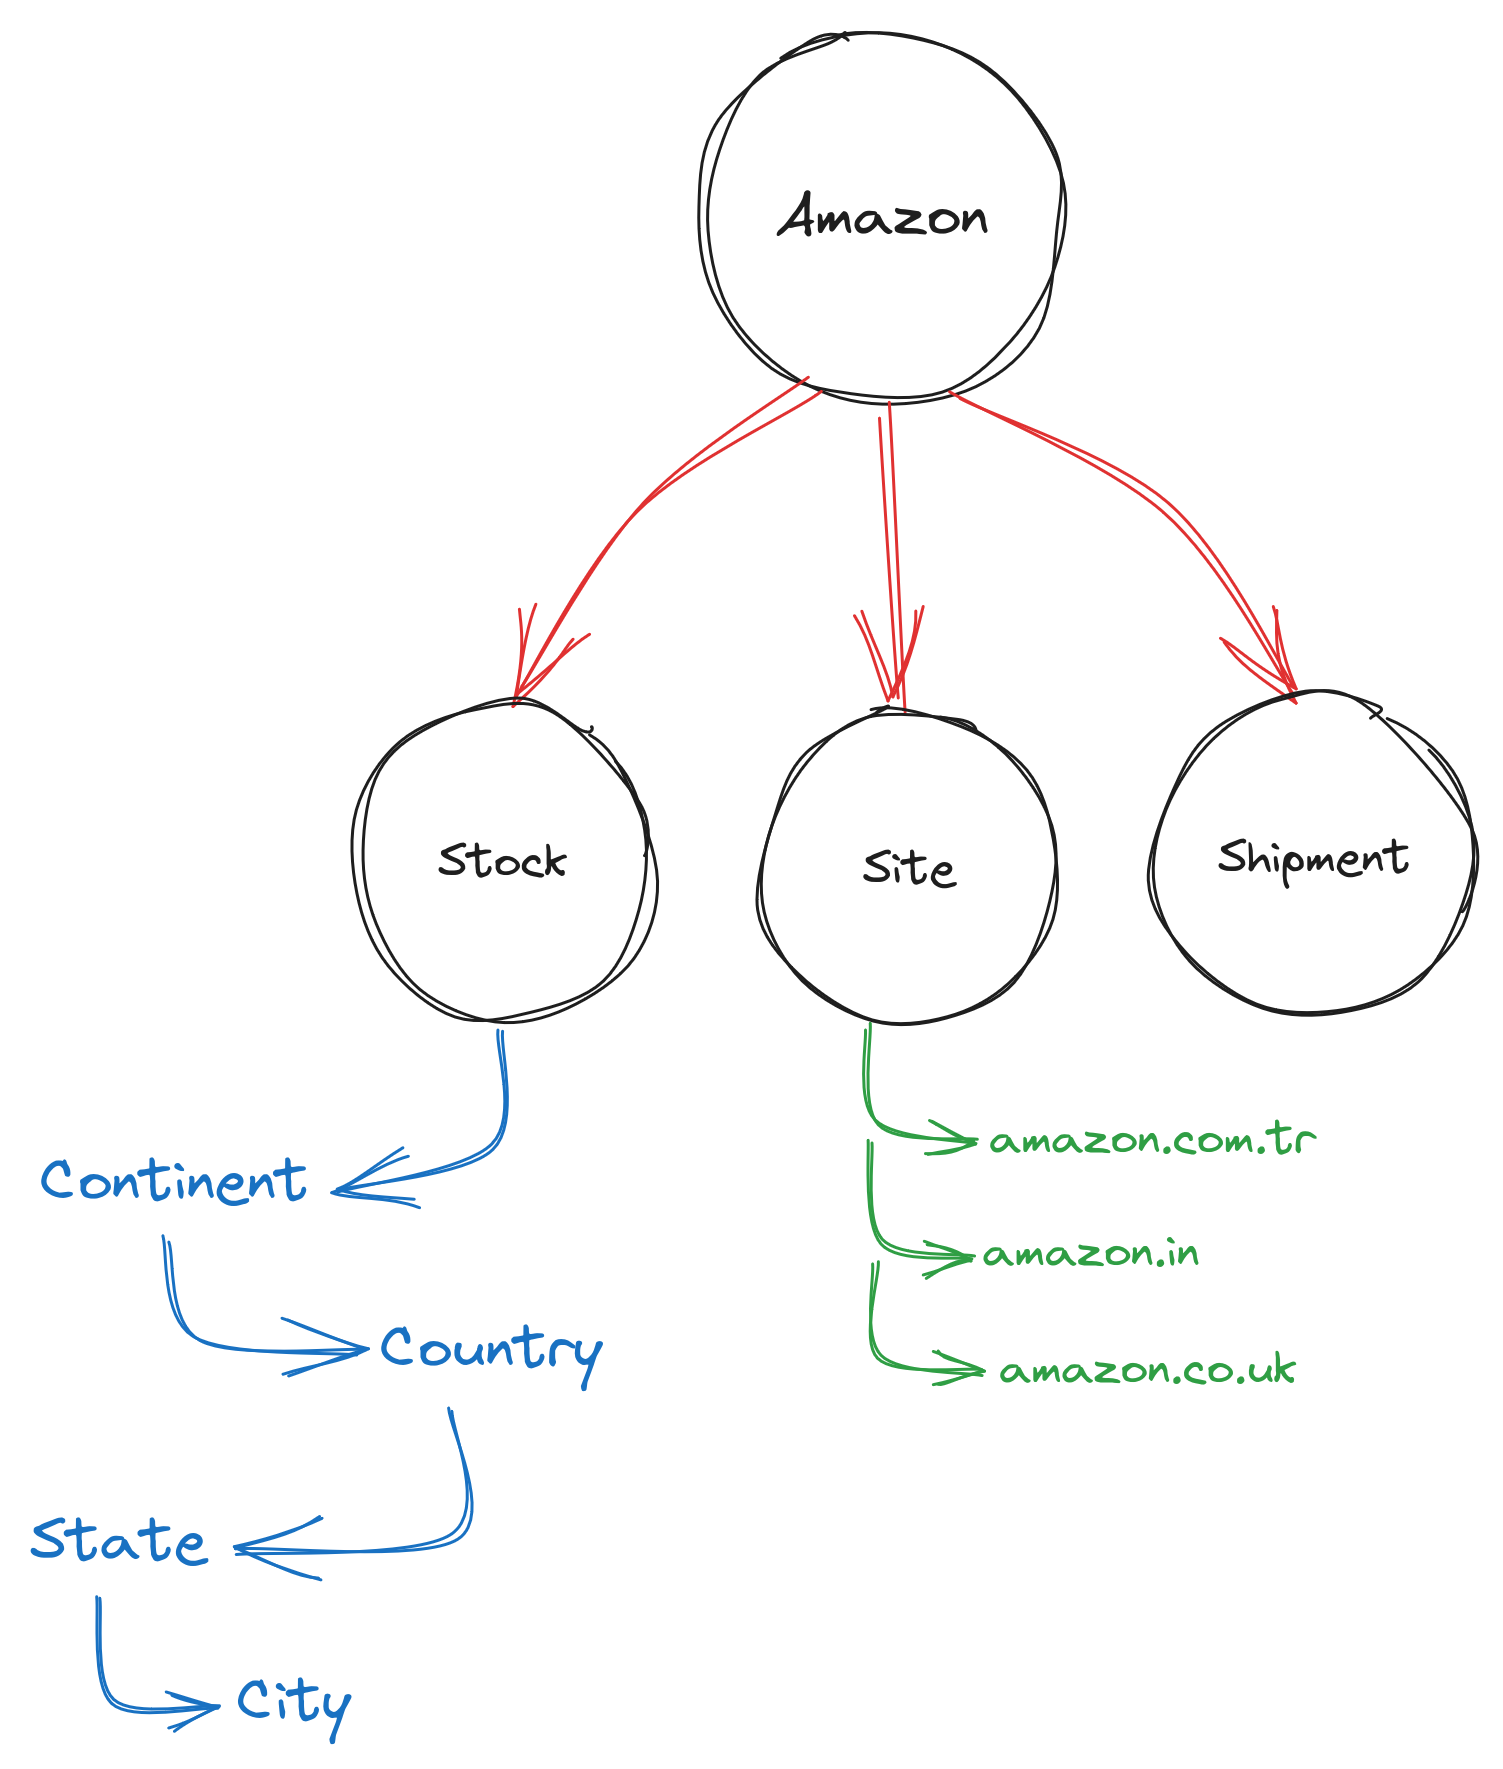
\includegraphics[width=0.85\textwidth, height=0.75\textheight]{../images/amazon-s3-comp(2)}
\end{center} 
\caption{ساختار کلی شرکت \lr{Amazon}}\label{amz-s3}
\end{figure}

\subsection{ارزش‌های قابل‌ اندازه‌گیری}\label{intro-movs}
با توجه به این تقسیم‌بندی انجام شده در \ref{amz-struct}، ارزش‌های قابل‌ اندازه‌گیری \label{movs}
و مهم برای شرکت \lr{Amazon} به شرح زیر می‌باشد:

\begin{itemize}
    \item  انبارداری \lr{(Stock)}
    
    \textbf{هدف اصلی} محصول باید در انبار‌هایی نزدیک محل تحویل باشد.
    \begin{itemize}
        \item 
        کالا‌ها باید در نزدیک‌ترین محل به مقصد ارسال کالا باشند (با \lr{km}\LTRfootnote{\lr{Kilometre}}سنجش می‌شود).
        
        \item 
        زمان پردازش و تحویل کالا به بخش ارسال کالا \lr{(Shipment)}، کمترین زمان ممکن باشد (با دقیقه و ساعت بررسی می‌شود).        
    \end{itemize}
    
    \item وبسایت \lr{Amazon} \lr{(Site)}
    
    \textbf{هدف اصلی} راحتی خرید
    \begin{itemize}
        \item سرعت بارگزاری وبسایت‌های \lr{Amazon} همه‌جا (با ثانیه بررسی می‌شود).
        
        \item 
        طراحی و تجربه‌ی کاربری \lr{(UI/UX)} (بازخورد‌های کیفی کاربران، برای مثال \textit{آیا این صفحه مفید بود} یا \textit{به صفحه‌ی \lr{x} چه امتیازی می‌دهید} و...)
    \end{itemize}

    \item ارسال کالا \lr{(Shipment)}
    
    \textbf{هدف اصلی} محصول سریع و سالم برسد
    \begin{itemize}
        \item 
        زمان تحویل کالا (با تعداد ساعت و روز بررسی می‌شود).
        \item 
        مسافت طی شده‌ی کالا (با \lr{km} سنجش می‌شود).
        
        \item 
        رضایت مشتری برای کالای تحویل داده شده (بازخورد‌های کیفی کاربران، برای مثال 
        \textit{به مامور تحویل چه امتیازی می‌دهید}،
        \textit{آیا کالا سالم است} و سوالاتی از این قبیل).
    \end{itemize}
\end{itemize}

\subsection{\lr{MOV}}

پروژه‌ی \lr{Amazon Analytics} به طور کلی، اگر به خوبی اجرا شود، می‌تواند بسیاری از هزینه‌های اضافی شرکت \lr{Amazon} را به صورت غیر مستقیم کاهش دهد.

برای مثال، در قسمت \lr{Stock}، با توجه به متریک‌های تعیین شده در \ref{intro-movs}، 
می‌تواند تاثیر مستقیمی به روی هزینه‌های قسمت \lr{Shipment} داشته باشد.

یا در قسمت \lr{Shipment} هر چقدر کارمندان تحویل مرسوله، بتوانند از مسیر‌های بهتر و کوتاه‌تر مرسوله‌ها را تحویل دهند، هزینه‌های جانبی ارسال برای \lr{Amazon} کاهش می‌یابد.

از طرفی تاثیراتی که بازخورد‌های مشتریان شرکت اگر مثمر ثمر واقع شوند، باعث رضایت بیشتر آنها شده و خرید‌‌های آنها به تبع آن، بیشتر شود که منجر به سود بیشتر 
\lr{Amazon}
می‌شود.
\subsubsection{در چه قسمت‌هایی پروژه باید به خوبی عمل کند؟}
\begin{itemize}
    \item 
    بتواند تحلیل و ارزیابیِ تمامی ارزش‌های قابل‌ اندازه‌گیری ذکر شده در \ref{intro-movs} را به مدیران رده‌بندی‌ شده بر اساس درخت سازمانی گزارش دهد.
    \item 
    بتواند با مقایسه‌ی عملکرد فعلی بخش‌های مختلف شرکت، میزان رشد و بهبود عملکرد آن را به صورت درصدی و دقیق گزارش دهد.
    \item
    مدیران شرکت علاوه‌ بر دسترسی به عملکرد بخش‌های مختلف شرکت، امکان دسترسی به بخش‌های کوچک و حتی هر کارمند را در صورت نیاز داشته باشد.
    
    \item 
    ارزیابی‌های انجام شده متناسب‌ با خروجی و عملکرد واقعی و قابل مشاهده‌ی شرکت باشد.
    
    \subsubsection{زمان تعیین شده برای \lr{MOV}}\label{time}
    پیش‌بینی می‌شود پروژه در سه تا پنج سال اول کار خود، بتواند به \lr{MOV} تعیین شده‌ی خودش برسد.
    \subsubsection{خلاصه‌} 
    به طور کلی این پروژه موفقیت‌آمیز خواهد بود اگر بتواند در زمان تعیین شده در \ref{time}
    هزینه‌های قسمت \lr{Stock} و 
    \lr{Shipment}
    را حدود ۱۵ تا ۲۰\% کاهش داده و میزان رضایت مشتری از قسمت \lr{Site} و تمام ۳ قسمت تعیین شده را حدود ۳۰ تا ۵۰\% افزایش بدهد.
\end{itemize}

\textbf{لازم به ذکر است}
که وظیفه و هدف پروژه صرفا ارزیابی آمار و تحلیل رشد و پیشبینی عملکرد شرکت خواهد بود، پس با این رویه مدیران و کارمندان شرکت \lr{Amazon}خودشان باید به فکر بهبود و ارتقای ارزش‌های قابل اندازه‌گیری ذکر شده باشند.


\section{جایگزین‌ها}
در این بخش، به بررسی جایگزین‌ها و راه‌حل‌های ممکن برای پیاده‌سازی \lr{Amazon Analytics} می‌پردازیم.

\subsection{گزارشات کتبی \lr{(Written Reports)}}\label{written-report}
در این راه‌حل هر کارمند در انتهای شیفت کاری، روز، ماه یا سال گزارشی از عملکرد خود یا بخشی که در آن کار می‌کند، به صورت کتبی به مدیر بخش ارائه می‌دهد. سپس مدیر بخش گزارشات دریافتی از کارمندان زیر دست خود را، جمع‌آوری، ارزیابی و تحلیل می‌کند و پس از آن عملکرد کلی بخش خود و زیردستان خود را به مدیران بالا دستی خود ارائه می‌دهد.
همین روند تا مدیران ارشد شرکت و سهام‌داران ادامه پیدا می‌کند.

\subsubsection{امکان‌سنجی}
    \begin{itemize}
        \item 
        اقتصادی
        
        این جایگزین براحتی با در اختیار قرار دادن کاغذ‌های مخصوص در اختیار کارمندان و مدیران، قابل انجام است.
        \item 
        تکنیکی
        
        این روش، هیچ نیاز مهم تکنیکالی ندارد. تنها نیاز آن با سواد بودن همه است که بتوانند گزارش را نوشته، و آن را بخوانند.
        \item 
        سازمانی
        
        از لحاظ سازمانی هم باید همه‌ی کارکنان توجیح شوند که گزارش خود را حتما بنویسند، و مدیران اطلاعات بخش خودشان را تحلیل کنند و به مدیران بالاتر ارائه دهند.
    \end{itemize}


\subsection{گزارشات دیجیتالی \lr{(Digital Reports)}}\label{half-digital}
در این روش، ثبت گزارشات \underline{با دست ولی به صورت الکترونیکی} صورت می‌پذیرد.
کارمندان گزارش عملکرد خود و بخش خود را به صورت دیجیتال به مدیران خود ارائه می‌دهند و به تبع آن، مدیران پس از تحلیل گزارشات دریافتی، نتایج آنها را هم به صورت دیجیتالی به مدیران ارشد و بالادستی خود ارائه می‌دهند.

\subsubsection{امکان‌‌سنجی}
    \begin{itemize}
        \item 
        اقتصادی
        
           این روش هم مانند \ref{written-report} آنچنان ریسک و یا احتمال انجام نشدن از لحاظ اقتصادی را ندارد.
        \item 
        تکنیکی
        
        از لحاظ تکنیکال، کارکنان و مدیران باید بتوانند برای ثبت و تحلیل داده‌ها، با تلفن همراه و یا رایانه براحتی کار کنند.
        \item 
        سازمانی
        
        این امکان‌سنجی هم برای این روش مانند \ref{written-report} است.
        
    \end{itemize}


\subsection{ارزیابی و تحلیل خودکار \lr{(Automated Reposts)}}\label{full-digital}
در این روش، تمامی داده‌ها و آمار‌های کارمندان، بخش‌ها و مدیران شرکت، به علاوه‌ی بازخورد‌های کاربران به صورت کاملا دیجیتالی و بدون دخالت دست انسان، جمع‌آوری شده و سپس تمامی تحلیل‌ها و ارزیابی‌های آنها در سیستم \lr{Amazon Analytics} انجام شده و به صورت کاملا طبقه بندی شده به تمامی مدیران ارائه می‌گردد.

\subsubsection{امکان‌سنجی}
    \begin{itemize}
        \item 
        اقتصادی
        
        این روش نیازمند سرمایه‌گذاری تقریبا عظیم شرکت \lr{Amazon} است تا بتوان آن را پیاده‌سازی کند. امکان‌پذیر هست اما نیاز به سرمایه‌ی زیادی دارد.
        \item 
        تکنیکی
        
        از لحاظ تکنیکال هیچ یک از کارکنان قرار نیست درگیر این سیستم شوند چون تمامی ثبت اطلاعات به صورت خودکار انجام می‌شود.
        \item 
        سازمانی
        
        اصولا چیزی میان کارکنان قرار نیست حس شود، اما مدیران با بتوانند از اطلاعاتی که سیستم \lr{Amazon Analytics} به خوبی استفاده کنند و برای بهبود قسمت‌های شرکت استفاده کنند و تصمیمات خوبی بگیرند.
    \end{itemize}

\subsection{بررسی یک مثال با راه‌حل‌های مختلف}
برای مثال می‌خواهیم تحویل یک کالا را از جهات مختلف بررسی کنیم.
\begin{itemize}
    \item راهکار \ref{written-report}
    
    مامور تحویل 
    \begin{enumerate*}
        \item 
        ساعت دریافت،
        \item 
        مسافت طی شده و 
        \item 
        ساعت تحویل کالا
    \end{enumerate*}
    را \textbf{شخصا} و به صورت \textbf{کتبی} پس از هر تحویل، در برگه‌ی گزارش روزانه‌ی خود مکتوب کرده و در پایان شیفت کاری، به مدیر بخش خود تحویل می‌دهد.
    
    سپس مدیر بخش، ارزیابی‌های مامورین مختلف را جمع‌آوری و تحلیل کرده و تمامی تحلیل‌های خود را به صورت \textbf{کتبی} به مدیران بالادستی خود ارائه می‌دهد.
    
    \item راهکار \ref{half-digital}
    
    مامور تحویل 
    \begin{enumerate*}
        \item 
        ساعت دریافت،
        \item 
        مسافت طی شده و 
        \item 
        ساعت تحویل کالا
    \end{enumerate*}
    را \textbf{شخصا} و به صورت \textbf{دیجیتالی} پس از هر تحویل، در برگه‌ی گزارش دیجیتالی روزانه‌ی خود ثبت کرده و در پایان شیفت کاری، برای مدیر بخش خود ارسال می‌کند.
    
    مدیر بخش در این روش، تحلیل‌ و آمار‌های دریافتی از کارمندان خودش را به صورت دیجیتال به مدیران بالادستی خود ارائه می‌دهد.
    
    در این روش برخلاف روش \ref{written-report} مدیران بالادستی درگیر تحلیل و آمار کاغذی نشده و از مزایای دیجیتالی بودن گزارشات (مثل دسته بندی راحت‌تر، قابلیت جستجو‌ی راحت‌تر و...) بهره‌مند می‌شوند.
    \item راهکار \ref{full-digital}
    
    زمانی که مامور تحویل، کالایی را برای تحویل به مشتری دریافت می‌کند، به صورت خودکار زمان دریافت کالا به مامور، مسافت طی شده و زمان تحویل کالا به مشتری، در سیستم ثبت شده و این آمار به صورت لحظه‌‌ای برای مدیران بالادستی قابل دسترسی می‌باشد.
    
    در این روش، دریافت اطلاعات، ارزیابی و تحلیل آنها به عهده‌ی سیستم است و هیچ کاربری در آن امکان دخالت ندارد. 
    
    در روش برخلاف \ref{half-digital} که وظیفه‌ی تحلیل آمار دریافتی به عهده‌ی مدیر بخش بود، تمامی تحلیل‌ها به صورت سیستمی انجام می‌شود و مدیران به راحتی به \textbf{خروجی} و \textbf{نتایج} تحلیل‌ها دسترسی آنی دارند.
    
\end{itemize}

\section{ارزش‌ها}
\subsection{هزینه‌ی کلی مالکیت \lr{TCO}}
\begin{itemize}
    \item 
    هزینه‌های مستقیم
    
    \begin{enumerate}
        \item 
        هزینه خرید و مستقرسازی سرور اصلی پردازش \lr{Amazon Analytics} و آماده‌سازی دیتابیس برای دریافت گزارشات و بایگانی آنها.
        
        اگر در ۳۰ نقطه از کره زمین بخواهیم سرور‌ها را قرار بدهیم و هر سرور ۲ میلیون دلار هزینه داشته باشد:
        \lr{\EyesDollar60,000,000} 
        
        \item 
        افزودن نظرسنجی‌های مختلف در جایگاه‌های مورد نیاز در قسمت \lr{Site}
        
        اگر برای پیاده‌سازی این کار نیاز به ۶ ماه کاری با ۲۵ روز کاری که هر روز کاری ۸ ساعت است و هزینه‌ی ساعتی یک توسعه‌دهنده‌ی \lr{Front-end} ساعتی ۱۲۰ دلار باشد:
        \begin{flushleft}
            \lr{$6 \times 25 \times 8 \times 120 =$ \EyesDollar144,000} 
        \end{flushleft}
        
        \item
        توسعه پلتفرم گزارش‌دهی و گزارش‌گیری و اجرای الگوریتم‌های ارزیابی موثر برای ارائه گزارش به مدیران:
        اگر برای پیاده‌سازی منطق این قسمت، نیاز به ۸ ماه کاری ۲۵ روزِ که هر روز کاری ۸ ساعت است و هزینه‌ی ساعتی یک توسعه‌دهنده‌ی \lr{Back-end} ساعتی ۱۵۰ دلار باشد:
        \begin{flushleft}
            \lr{$8 \times 25 \times 8 \times 150 =$ \EyesDollar 240,000} 
        \end{flushleft}
        
        و برای پیاده‌سازی رابط کاربری نیاز به ۴ ماه کاری ۲۵ روزِ که هر روز کاری ۸ ساعت است و هزینه‌ی ساعتی یک توسعه‌دهنده‌ی \lr{Front-end} ساعتی ۱۲۰ دلار باشد:
        \begin{flushleft}
            \lr{$4 \times 25 \times 8 \times 120 =$ \EyesDollar 96,000} 
        \end{flushleft}
        
        که در کل 
        \lr{\EyesDollar336,000}
        هزینه‌ی این قسمت می‌شود.
    \end{enumerate}
    
    
    \item 
    هزینه‌های آتی
    
    \begin{enumerate}
        \item 
        پشتیبانی مداوم سرورها برای بایگانی صحیح اطلاعات (دور ریختن اطلاعات به درد نخور و مدیریت فضا و پهنای باند سرور)
        
        اگر برای هر ۳۰ سرور، یک مختصص \lr{DevOps} با حقوق ۴۰ در هر ساعت برای ۱۵ روز کاری استخدام شود (برای یک ماه به دو متخصص نیاز داریم):
        \begin{flushleft}
            \lr{$2 \times (30 \times 1 \times 40 \times 15 \times 8) =$ \EyesDollar 228,000 per month} 
        \end{flushleft}
        
        \item 
        توسعه و بهبود مداوم الگوریتم‌های ارزیابی عملکرد
        
        اگر برای هر قسمت از شرکت، یک \lr{Machine Learning Engineer} در رده‌ی \lr{Senior} استخدام کنیم در هر سال:
        \begin{flushleft}
            \lr{$3 \times 375000=$ \EyesDollar 1,125,000}
        \end{flushleft}
        
        \item 
        بهبود روش‌های دریافت نظر کاربران از محصولات و شرکت
        
        اگر یک تیم ۵ نفره بخواهند در مجموع، ۶ ماه از یک سال را کار کنند، و به طور میانگین حقوق‌شان ۱۰۰ دلار در ساعت باشد، سالینه:
        \begin{flushleft}
            \lr{$5 \times 100 \times 6 \times 25 \times 8 =$ \EyesDollar 600,000}
            
        \end{flushleft}
    \end{enumerate}
    
    
    \item 
    هزینه‌های غیر مستقیم
    
    به دلیل خودکار بودن سیستم پیشنهادی و عدم دخالت کارکنان نیازی به هزینه‌هایی چون عدم بهره‌وری اولیه، تضمین کیفیت، آموزش موارد این چنینی وجود ندارد و کارکنان مانند سابق کار خود را انجام می دهند و تنها تفاوت ایجاد شده این است که در حین عملکرد به صورت خودکار داده هایی از انها در سرور ارزیابی ذخیره می شود.
    
    تنها آموزشی که نیاز‌ است، آموزشی به مدیران بخش‌هاست که برای استفاده از گزارش‌ها و سیستم تازه ایجاد شده باید آموزش ببینند که هزینه‌ای را در کل در بر نمیگیرد.
    
\end{itemize}
\subsection{مزایای کلی مالکیت \lr{TBO}}
\begin{enumerate}
    \item 
    شناسایی و تقسیم‌بندی کارکنان بر اساس نحوه و بازدهی کارکرد برای تعیین پاداش و حقوق عادلانه
    \item 
    تحلیل عملکرد کلی شرکت برای بررسی رشد یا سقوط و یافتن هرچه سریع‌تر موارد قوت و ضعف
    \item 
    امکان دسترسی مدیران ارشد به گزارشات در سطح‌های مختلف اداری برای اطمینان از عملکرد مدیران میانی 
    \item 
    باعث بهبود در تصمیم‌گیری می شود، به طور مثال اگر بدانیم کارکنان در چه کارهایی قوت و یا ضعف دارن امکان مدیریت بهتری برای کارکنان و فعالیت های آنان انجام میدهیم یا وقتی بدانیم انبار در کجا کافی نیست انبار را گسترش و یا انبار جدیدی اضافه می کنیم.
\end{enumerate}

\section{تحلیل جایگزین‌ها}
در این قسمت به بررسی راه‌حل‌های ارائه می‌پردازیم و جنبه‌های متفاوت‌ آنها را بررسی می‌کنیم.

\begin{itemize}
\item         
روش‌های جمع‌آوری داده
\begin{itemize}
    \item راهکار \ref{written-report} 
    
    کاملا دستی، و به صورت پایین به بالا انجام می‌شود.
  
  در این روش، تا زمانی که کارمندی گزارشات خود را مکتوب نکرده و تحویل نداده، هیچ مدیری به هیچ داده‌ی جدیدی دسترسی نداشته؛ به علاوه گزارشات دریافتی از کارمندان و تحلیل‌ها میتوانند کاملا غیرواقعی‌ باشند.
    \item راهکار \ref{half-digital}
    
    ارائه گزارشات اولیه و عملکرد پایه‌ای هر کارمند به صورت دستی ولی دیجیتال و پایین به بالا انجام می‌شود.
    
    در این روش برخلاف روش \ref{written-report} گزارشات دیجیتال دریافت می‌شوند اما همانند روش \ref{written-report} تا زمانی که کارمندی گزارشات خود را ثبت نکرده، هیچ مدیری به هیچ داده‌ی جدیدی دسترسی ندارد. به علاوه، در این روش چون ثبت اطلاعات به صورت دیجیتال صورت می‌گیرد، دسترسی به گزارشات گذشته راحت‌تر و دقیق‌تر از روش \ref{written-report} است.
    
    \item راهکار \ref{full-digital}
    
    تمامی آمار و اطلاعات به صورت خودکار توسط سیستم محاسبه و ثبت می‌شود و کاربر هیچ دخالتی در آن ندارد.
    
    در این روش، امکان جعل آمار و تغییر آن به هیچ عنوان وجود ندارد و مدیران (در صورت نیاز) به صورت تماما لحظه‌ای، می‌توانند ارزیابی و گزارشات آماری و عملکرد کارمندان و بخش‌های مختلف شرکت را از سیستم دریافت کنند.
\end{itemize}
\item         
متریک‌های مورد استفاده

تمامی این متریک‌ها در \ref{intro-movs} و در تصویر \ref{amz-comp} تعریف شده‌اند.

\begin{figure}[b]
    \begin{center}
        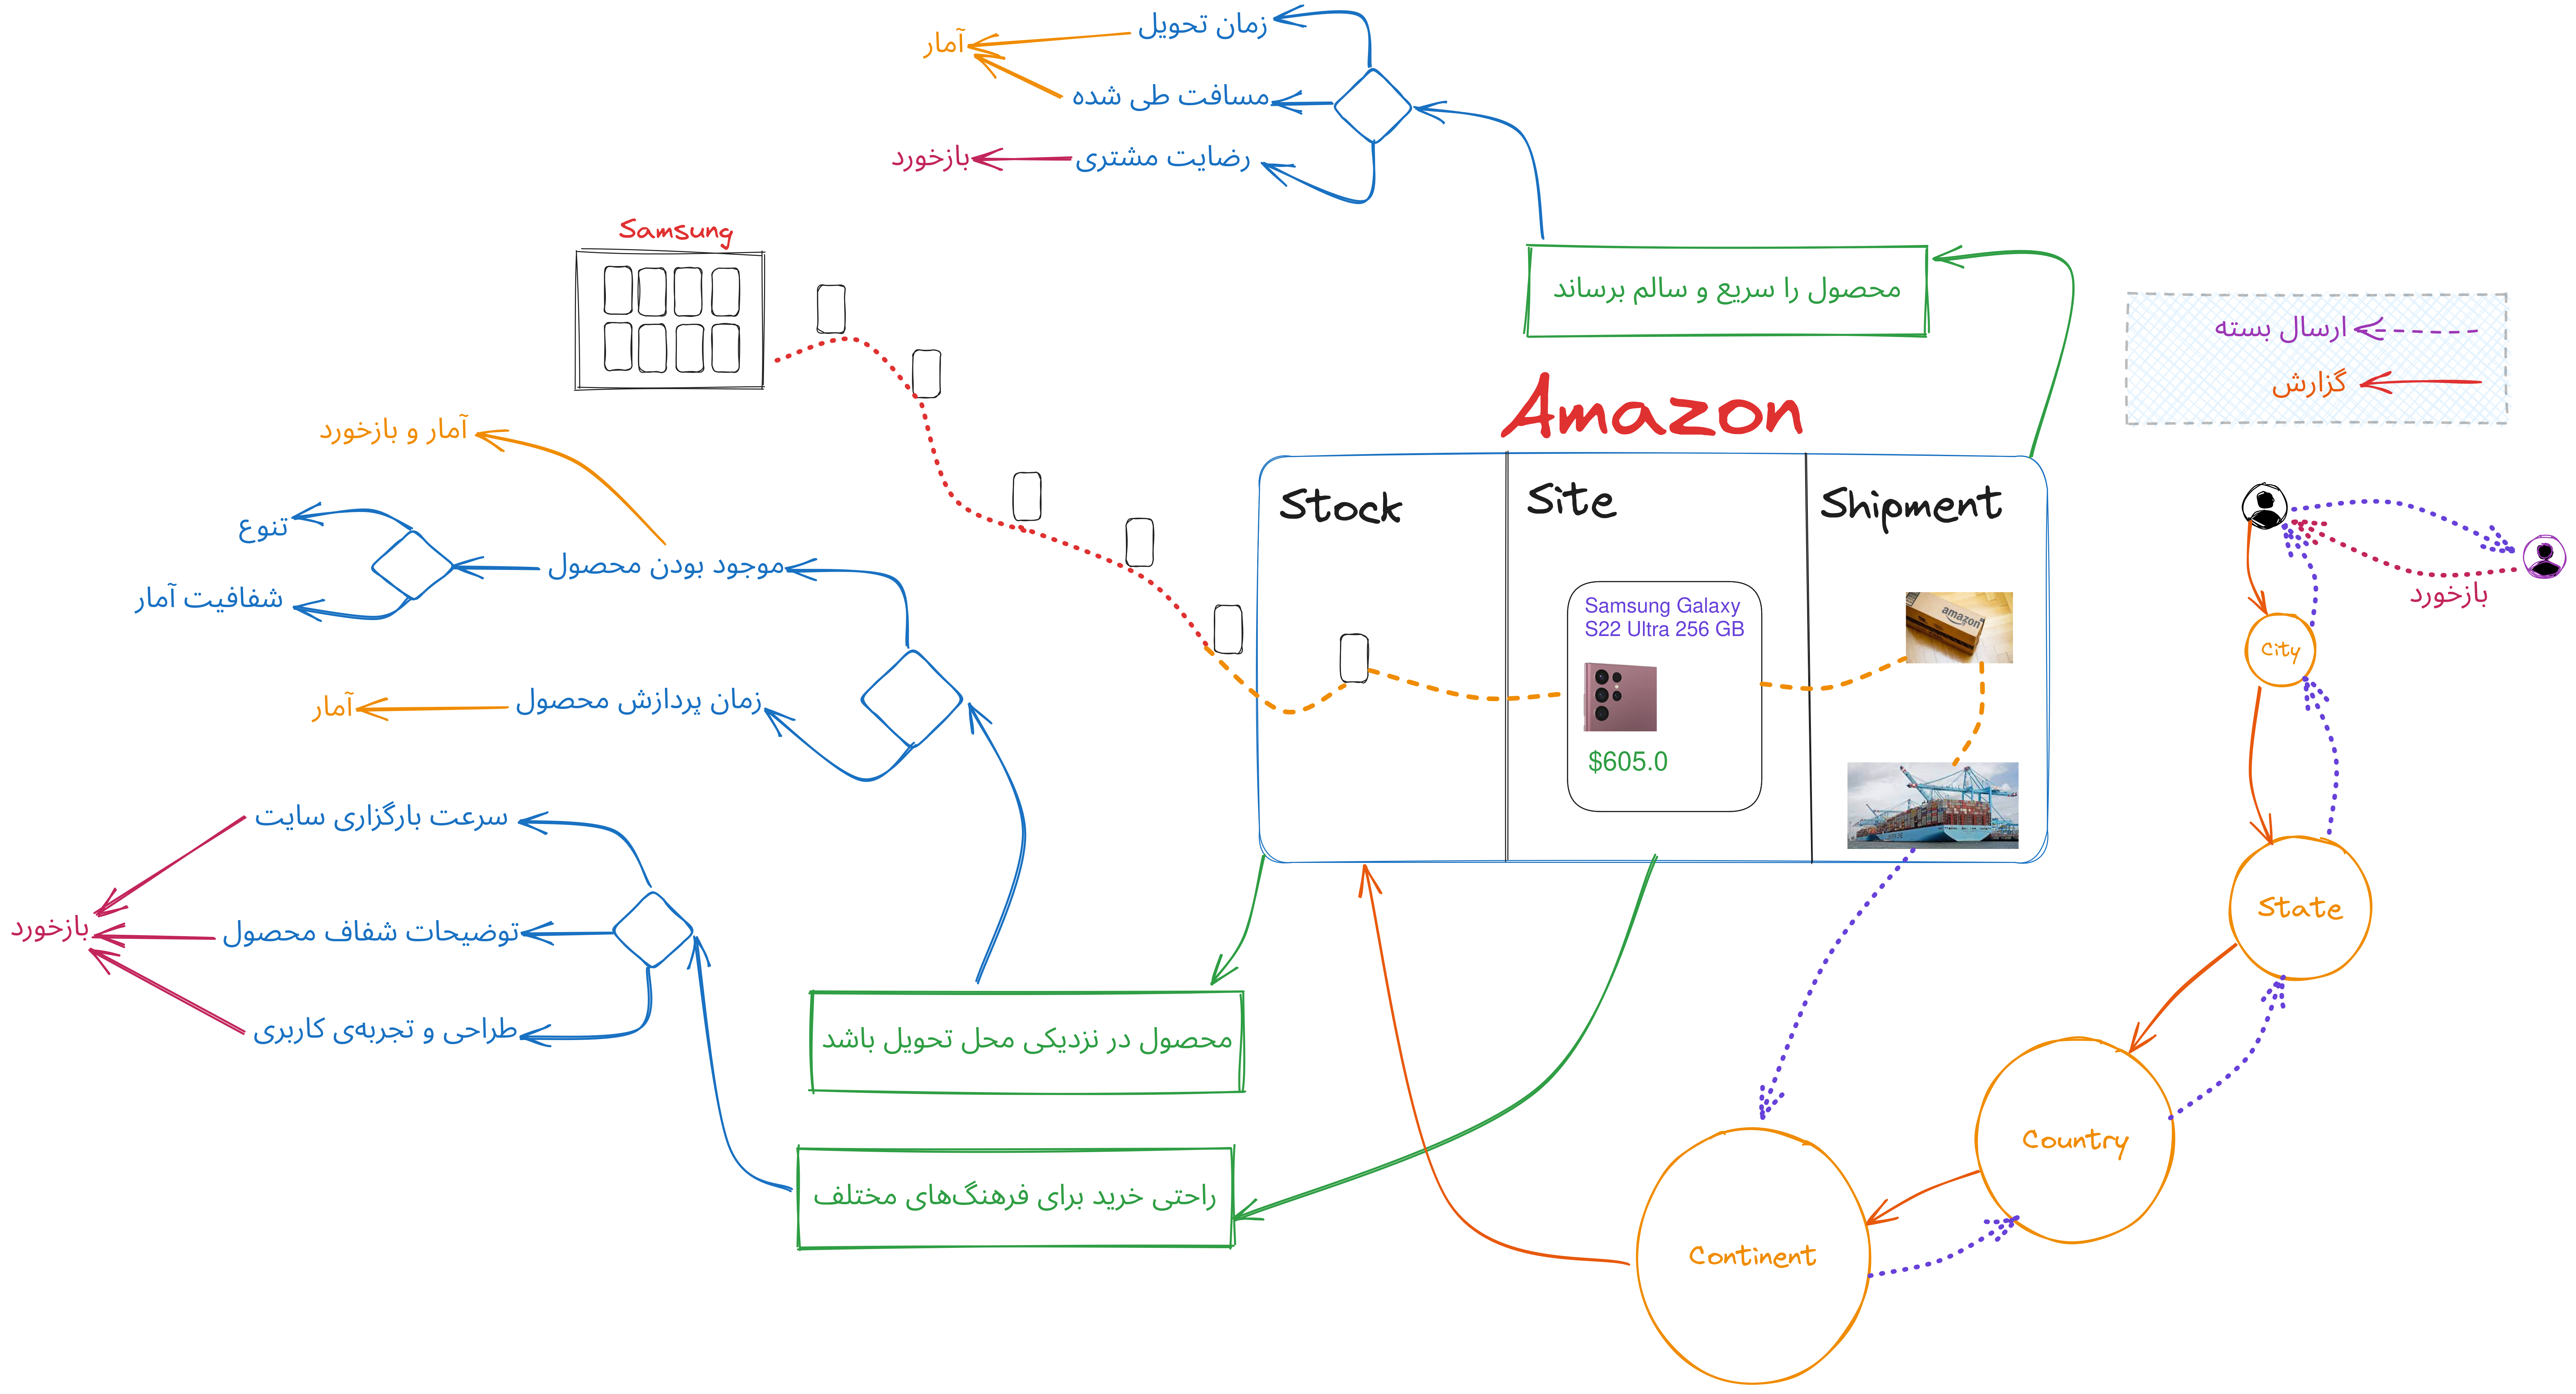
\includegraphics[width=0.95\textheight, height=0.95\textwidth, angle=90]{../images/amazon-comp(2)}
    \end{center}
\caption{ارزش‌ها و متریک‌های مهمِ \lr{Amazon Analytics}}\label{amz-comp}
\end{figure}
\end{itemize}

\subsection{ارائه نتایج بررسی و مقایسه}
\subsubsection{ماتریس تصمیم‌گیری راهبردی}

\begin{table}[H]\caption{\lr{Does the strategy meet the required objectives?}}
    \begin{latin}
        \begin{center}
            \begin{adjustbox}{width=\textwidth}
                \begin{tabular}{|M{4cm}|M{4cm}|M{4cm}|c|}
                    \hline
                    \multirow{2}{*}{Required Objectives}
                    & \multicolumn{3}{|c|}{Strategies} \\
                    \cline{2-4}
                    & Written Reports (\ref{written-report}) & Digital Reposts (\ref{half-digital}) & Automated Reports (\ref{full-digital}) \\
                    \hline
                    \rl{دسترسی به عملکرد همه بخش‌ها توسط مدیران} & Yes, but hard & Yes  & Yes \\
                    \hline
                    \rl{دسترسی به گزارشات قدیمی} & Yes, but hard & Yes & Yes \\
                     \hline
                    \rl{مصورسازی تحلیل‌ها} & Yes, but hard & Yes & Yes \\
                    \hline
                    \rl{دقت در گزارشات} & Yes, but not guaranteed & Yes, but not guaranteed & Yes \\
                    \hline
                    \rl{گزارشات بهبود عملکرد} & Yes, but hard & Yes & Yes \\
                    \hline
                    \rl{اعتبار ارزیابی} & Yes, but low & Yes, but low & Yes \\
                    \hline
                     \rl{دریافت گزارش عملکرد در بازه‌های کوتاه مدت و یا آنی} &  No & Yes, but if user submits them quickly & Yes \\
                    \hline
                \end{tabular}
            \end{adjustbox}
        \end{center}
    \end{latin}
\end{table}

\begin{table}[H]\caption{\lr{How likely is this strategy to meet the other objectives?}}
    \begin{latin}
        \begin{center}
            \begin{adjustbox}{width=\textwidth}
                \begin{tabular}{|M{5cm}|c|c|c|c|}
                    \hline
                    \multirow{2}{*}{Other objectives} &
                    \multirow{2}{*}{Importance} &
                    \multicolumn{3}{|c|}{Strategies}\\
                    \cline{3-5}
                    & & Written Reports & Digital Reports & Automated Reports  \\
                    \hline
                    \rl{دسترسی به گزارشات همه‌ی بخش‌ها}
                    & 5
                    & - 
                    & 5
                    & 5 \\
                    \hline
                    \rl{جستجو در گزارشات بایگانی شده}
& 4
& - 
& 5
& 5 \\
\hline
                    \rl{ارائه و مصورسازی عملکردها}
& 3
& - 
& 3
& 5 \\
\hline
                    \rl{دقت در داده‌های دریافتی}
& 5
& - 
& 2
& 5 \\
\hline

                              \rl{دسترسی لحظه‌ای به گزارشات و ارزیابی‌ها}
  & 3
  & - 
  & 2
  & 5 \\
  \hline
          
                              \rl{هزینه‌، زمان و منابع صرف شده برای هر ارزیابی}
& 2
& - 
& 2
& 5 \\
\hline
                    \textbf{\rl{\textbf{مجموع}}} & & 0 & 74 & 110 \\
                    \hline
                \end{tabular}
            \end{adjustbox}
        \end{center}
    \end{latin}
\end{table}

ما نمی‌توانستیم از منطق صفر و یکی برای تحلیل‌ راه‌حل‌های انتخاب شده در ماتریس تصمیم‌گیری راهبردی استفاده کنیم و برای همین از الفاظی که در جدول استفاده شده‌اند استفاده کرده‌ایم. به تبع همین، در دومین جدول هم مجموعه‌ای ردیف‌های جدول اول را آوردیم تا بتوانیم به خوبی به آنها نمره بدهیم.

\subsubsection{جایگزین‌ پیشنهادی}
با توجه به مزایای روش 
\ref{full-digital}
و نمرات آن، پیشنهاد ما استفاده از این روش برای پیاد‌ه‌سازی 
\lr{Amazon Analytics}
است.
\subsection{ماتریس \lr{RACI}}
\begin{table}[H]
    \begin{latin}
        \begin{center}
            \begin{tabular}{|c|c|c|c|c|}
                \hline
                Task/Person & Mahdi & Mohammad & Teacher & TA \\
                \hline
                \rl{بارش فکری} & R & R/A & - & - \\
                \hline
                \rl{ساختار بندی شرکت \lr{Amazon}} & R& R/A & - & -\\
                \hline
                 \rl{چینش چارت سازمانی} & R/A & R & - & - \\
                 \hline
                 \rl{ساختار بندی پروژه بر اساس ساختار شرکت} &R/A& R& - & - \\
                \hline
                \rl{یافتن ارزش‌های قابل اندازه‌گیری} & R & R/A & C & -\\
                \hline
                                 \rl{یافتن \lr{MOV}های شرکت} & R & R/A & C & - \\
                \hline
                \rl{یافتن \lr{MOV}های پروژه} & R/A & R & C & - \\
                \hline
                
                 \rl{یافتن و امکان‌سنجی جایگزین‌ها} & R & R/A & - & -\\
                \hline
                
                \rl{بررسی \lr{TCO}} & R/A & R & - & C\\
                \hline
                \rl{بررسی \lr{TBO}} & R & R/A & - & C \\
                \hline
                
                 \rl{تحلیل و بررسی جایگزین‌ها} & R/A & R & - & - \\
                  \hline
                  \rl{نوشتن ماتریس تصمیم‌گیری راهبردی} & R& R/A& - & -\\
                  \hline
                  \rl{نوشتن ماتریس \lr{RACI}} & R/A& R& C& - \\
                  \hline
                  \rl{نوشتن سند پروژه} & R/A & I & - & - \\
                  \hline
                  \rl{نوشتن قالب بارش فکری} & R & R/A & - & - \\
                  \hline
            \end{tabular}
        \end{center}
    \end{latin}
\end{table}
\end{document}